% Generated by julia/scripts/generate_manuscript_numerical_artifacts.jl.
% Sources: financial_terminal_audit_uncertainty.csv and financial_annual_walkforward_audit_uncertainty.csv.
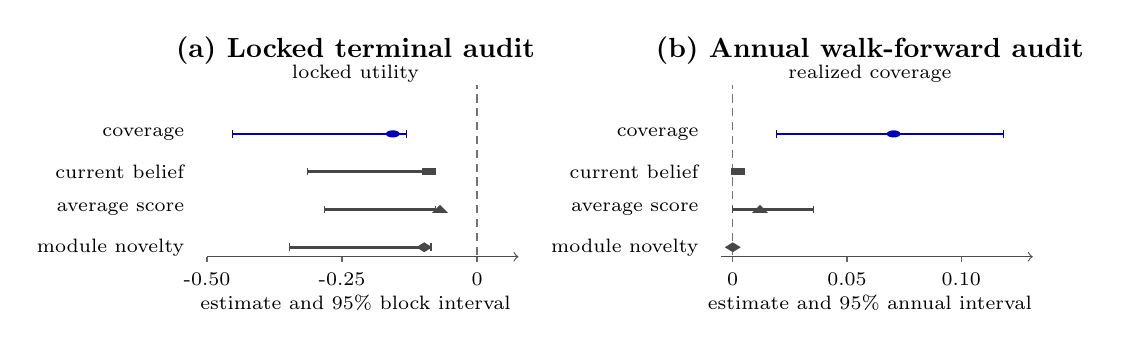
\begin{tikzpicture}[x=0.92cm,y=0.48cm,font=\scriptsize]
  \node[font=\bfseries] at (4.05,5.45) {(a) Locked terminal audit};
  \node at (4.05,4.85) {locked utility};
  \node[font=\bfseries] at (11.15,5.45) {(b) Annual walk-forward audit};
  \node at (11.15,4.85) {realized coverage};
  \draw[black!55,densely dashed] (5.727273,0.05) -- (5.727273,4.55);
  \draw[black!55,densely dashed] (9.257692,0.05) -- (9.257692,4.55);
  \draw[blue!72!black,line width=0.9pt] (2.349676,3.25) -- (4.757297,3.25);
  \draw[blue!72!black] (2.349676,3.15) -- (2.349676,3.35);
  \draw[blue!72!black] (4.757297,3.15) -- (4.757297,3.35);
  \fill[blue!72!black] (4.564722,3.25) circle (0.095);
  \node[anchor=east] at (1.82,3.25) {coverage};
  \draw[black!72,line width=0.9pt] (3.387103,2.25) -- (5.148218,2.25);
  \draw[black!72] (3.387103,2.15) -- (3.387103,2.35);
  \draw[black!72] (5.148218,2.15) -- (5.148218,2.35);
  \fill[black!72] (4.973837,2.16) rectangle (5.153837,2.34);
  \node[anchor=east] at (1.82,2.25) {current belief};
  \draw[black!72,line width=0.9pt] (3.624146,1.25) -- (5.155993,1.25);
  \draw[black!72] (3.624146,1.15) -- (3.624146,1.35);
  \draw[black!72] (5.155993,1.15) -- (5.155993,1.35);
  \fill[black!72] (5.216539,1.37) -- (5.106539,1.16) -- (5.326539,1.16) -- cycle;
  \node[anchor=east] at (1.82,1.25) {average score};
  \draw[black!72,line width=0.9pt] (3.141269,0.25) -- (5.092602,0.25);
  \draw[black!72] (3.141269,0.15) -- (3.141269,0.35);
  \draw[black!72] (5.092602,0.15) -- (5.092602,0.35);
  \fill[black!72] (4.997946,0.38) -- (4.887946,0.25) -- (4.997946,0.12) -- (5.107946,0.25) -- cycle;
  \node[anchor=east] at (1.82,0.25) {module novelty};
  \draw[blue!72!black,line width=0.9pt] (9.855796,3.25) -- (13.00087,3.25);
  \draw[blue!72!black] (9.855796,3.15) -- (9.855796,3.35);
  \draw[blue!72!black] (13.00087,3.15) -- (13.00087,3.35);
  \fill[blue!72!black] (11.478529,3.25) circle (0.095);
  \node[anchor=east] at (8.92,3.25) {coverage};
  \draw[black!72,line width=0.9pt] (9.257692,2.25) -- (9.41809,2.25);
  \draw[black!72] (9.257692,2.15) -- (9.257692,2.35);
  \draw[black!72] (9.41809,2.15) -- (9.41809,2.35);
  \fill[black!72] (9.226471,2.16) rectangle (9.406471,2.34);
  \node[anchor=east] at (8.92,2.25) {current belief};
  \draw[black!72,line width=0.9pt] (9.257692,1.25) -- (10.368312,1.25);
  \draw[black!72] (9.257692,1.15) -- (9.257692,1.35);
  \draw[black!72] (10.368312,1.15) -- (10.368312,1.35);
  \fill[black!72] (9.633211,1.37) -- (9.523211,1.16) -- (9.743211,1.16) -- cycle;
  \node[anchor=east] at (8.92,1.25) {average score};
  \draw[black!72,line width=0.9pt] (9.257692,0.25) -- (9.257692,0.25);
  \draw[black!72] (9.257692,0.15) -- (9.257692,0.35);
  \draw[black!72] (9.257692,0.15) -- (9.257692,0.35);
  \fill[black!72] (9.257692,0.38) -- (9.147692,0.25) -- (9.257692,0.12) -- (9.367692,0.25) -- cycle;
  \node[anchor=east] at (8.92,0.25) {module novelty};
  \draw[->,black!70] (2.0,0) -- (6.3,0);
  \draw[->,black!70] (9.1,0) -- (13.4,0);
  \foreach \value/\label in {-0.5/{-0.50},-0.25/{-0.25},0/{0}} {
    \pgfmathsetmacro{\xp}{2.0+4.1*(\value+0.5)/0.55}
    \draw[black!60] (\xp,0) -- (\xp,-0.13);
    \node[anchor=north] at (\xp,-0.18) {\label};
  }
  \foreach \value/\label in {0/{0},0.05/{0.05},0.10/{0.10}} {
    \pgfmathsetmacro{\xp}{9.1+4.1*(\value+0.005)/0.13}
    \draw[black!60] (\xp,0) -- (\xp,-0.13);
    \node[anchor=north] at (\xp,-0.18) {\label};
  }
  \node[anchor=north] at (4.05,-0.75) {estimate and 95\% block interval};
  \node[anchor=north] at (11.15,-0.75) {estimate and 95\% annual interval};
\end{tikzpicture}
